Consider the following system:

\begin{center}
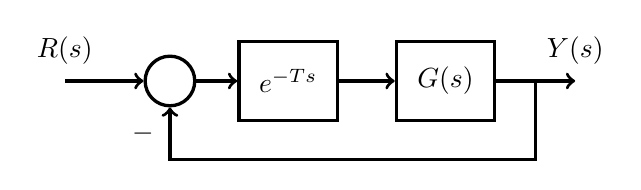
\begin{tikzpicture}[very thick,
sysblock/.style={draw,rectangle,inner sep=6pt,minimum width=1.25cm,minimum height=1.0cm,very thick},
summer/.style={circle,draw,very thick}]
\draw (0,0) node[summer] (sum) {\rule{10pt}{0pt}};
\draw (1.5,0) node[sysblock] (C) {$e^{-Ts}$};
\draw (3.5,0) node[sysblock] (G) {$G(s)$};
\draw[<-] (sum.180) -- ++(-1,0) node[above=2pt] {$R(s)$};
\draw[->] (sum.0) -- (C.180);
\draw[->] (C.0) -- (G.180);
\draw[->] (G.0) -- ++(0.5,0) |- ++(0,-1)  -| (sum.-90) node[below left=2pt] {$-$};
\draw[->] (G.0) ++(0.5,0) -- ++(0.5,0) node[above=2pt] {$Y(s)$};

\end{tikzpicture}
\end{center}

\noindent From the Bode plot of $G(s)$ below, what delay can be tolerated before the system becomes unstable?  Perform multiplication and division to reduce your answer to a single number.  Represent your answer in seconds.
\vspace{0.3in}

\begin{flushright}
%\includegraphics[trim=2.5cm 0 0 0]{./Problem12fig.pdf}
\includegraphics[trim=2.5cm 0 0 0]{\mainfolder/LectureNotes/\lecturefolder/HomeworkProblems/Problem11figure}
\end{flushright}

